\chapter{РАЗРАБОТКА И ТЕСТИРОВАНИЕ СЕРВИСА АНАЛИЗА НОВОСТЕЙ}
\aftertitle

\section{Выбор стека технологий}

Перед началом разработки системы анализа новостей был произведен анализ различных технологий и выбор стека технологий для разработки сервиса. Выбор основного компонента сервиса ~-- векторной базы данных ~-- был осуществлен в главе \ref{chap:arch_design}.

\subsection{Выбор языка программирования}

В качестве языка программирования для разработки системы анализа новостей был выбран Python. Выбор Python в качестве основного языка программирования для разработки системы анализа новостей обусловлен несколькими важными причинами.

Python является лидирующим языком в области науки о данных и машинного обучения. Большинство библиотек для этих задач написаны на Python или имеют привязки к нему.

Python является простым и высокоуровневым языком, который позволяет разрабатывать сложные системы, затрачивая меньше усилий, по сравнению со многими другими языками. Python отличается от других языков своей простотой и читаемостью. Это ускоряет процесс разработки, облегчает отладку и поддержку кода.

Python имеет множество фреймворков для разработки веб-сервисов, таких как FastAPI, Flask и Django, что делает его идеальным выбором для создания веб-сервиса, предусмотренного в этом проекте.

\subsection{Выбор фреймворка для создания REST API}

Для реализации веб-сервиса нужно выбрать какой-либо фреймворк для разработки веб-приложений. В данной работе необходимо реализовать RESTful-сервис. Были сформулированы следующие требования к фреймворку:
\begin{itemize}
    \item поддержка реализации REST API;
    \item простота разработки и минимальное количество шаблонного кода;
    \item поддержка валидации входящих данных;
    \item поддержка создания документации в формате swagger.
\end{itemize}


Выбор подходящего фреймворка для реализации REST API в веб-сервисе зависит от многих факторов. Были рассмотрены преимущества и недостатки Django, Flask и FastAPI для данного проекта.

Django ~-- это высокоуровневый фреймворк разработки веб-приложений на Python, который обеспечивает полный набор функциональности <<из коробки>>. Django предлагает ряд модулей для различных задач, включая аутентификацию, формы, маршрутизацию, управление сессиями и взаимодействие с базами данных. Django следует принципу DRY (Don't Repeat Yourself) и призывает к максимальному повторному использованию кода.

Преимущества:
\begin{itemize}
    \item обширная функциональность: Django имеет встроенные модули для работы с базами данных, административную панель, систему шаблонов и многое другое, что позволяет сократить время разработки;
    \item большое сообщество пользователей, что позволяет получить поддержку и множество ресурсов для изучения.
\end{itemize}

Недостатки:
\begin{itemize}
    \item избыточность: Django ~-- фреймворк, предназначенный для создания крупных веб-приложений со множеством функций, которые избыточны для REST сервиса;
    \item отсутствие некоторых функций для работы с REST API, таких как поддержки валидации данных и автоматической генерации документации Swagger.
\end{itemize}

Flask ~-- это фреймворк для разработки веб-приложений на Python. Он предназначен для создания небольших и простых веб-сайтов и API. В отличие от Django, Flask не предлагает множество функций <<из коробки>>, но предоставляет основу, на которой можно строить, используя расширения. Flask предлагает больше гибкости, позволяя разработчикам выбирать инструменты и библиотеки, которые они хотят использовать.

Преимущества:
\begin{itemize}
    \item гибкость и модульность: Flask позволяет выбирать и использовать только те компоненты, которые действительно необходимы для проекта;
    \item простота использования: Flask легко изучить и начать использовать, особенно для небольших проектов.
\end{itemize}

Недостатки:
\begin{itemize}
    \item при создании REST API с Flask может потребоваться больше шаблонного кода по сравнению с другими фреймворками.
    \item отсутствие встроенной валидации данных, что может усложнить процесс разработки REST API.
\end{itemize}

FastAPI ~-- это современный, высокопроизводительный веб-фреймворк для построения API с Python. Он обеспечивает автоматическую генерацию документации для API, валидацию данных с помощью Python Type Hints и поддерживает асинхронные запросы. FastAPI был разработан с упором на удобство использования и производительность.

Преимущества:
\begin{itemize}
    \item FastAPI обеспечивает высокую производительность.
    \item встроенная валидация данных: FastAPI поддерживает валидацию данных на основе Python type hints, что облегчает проверку входящих данных.
    \item автоматическая генерация документации Swagger: FastAPI автоматически генерирует документацию Swagger на основе кода, что облегчает создание и поддержку документации API.
\end{itemize}

Недостатки:
\begin{itemize}
    \item FastAPI наименее популярный фреймворк, имеющий меньшее количество обучающих материалов.
\end{itemize}

Исходя из рассмотренных преимуществ и недостатков, для разработки проекта был выбран фреймоврк FastAPI. Он обеспечивает быстродействие и простоту использования, встроенную валидацию данных и генерацию документации Swagger, что полностью соответствует требованиям к фреймворку для этого проекта.

\section{Разработка системы добавления данных в векторную БД}

С помощью парсера новостные данные собираются и сохраняются в базе данных SQLite. Чтобы работать с ними, их необходимо проанализировать, очистить от выбросов и добавить в векторную базу данных Weaviate.

Для построения RESTful-сервиса требуется разработать скрипты: скрипт для анализа и предобработки данных и скрипт для добавления новостей в Weaviate.

Для анализа и предобработки данных использовался язык программирования Python и библиотеки pandas, numpy и matplotlib. Это широко распространенные инструменты, применяемые в Data Science и при работе с данными, которые позволяют быстро выполнять множество различных операций, связанных с анализом и предобработкой данных.

В первую очередь, требуется определить временные рамки собранных новостей. В рамках работы, были собраны новости с 2019-04-23 по 2020-12-07. Т.к. собрано небольшое количество данных с новостных лент, то не представляет трудностей считать все данные в оперативную память и удобным образом работать с ними, используя средства библиотеки pandas, такие как DataFrame.

Следующим этапом предобработки данных является анализ распределения количества новостей за день. Это позволит выявить ошибки и аномалии в данных, такие как аномально маленькое или аномально большое количество новостей в день, что может свидетельствовать о каких-либо ошибках в сборке данных. До определенной даты количество новостей существенно меньше, чем после этой даты. Изначально собиралось по несколько новостей, максимум, несколько десятков новостей в день. Затем собирались от тысячи до двух тысяч новостей в день. Такая большая разница в количестве новостей в день может привести в дальнейшем к нарушению работы алгоритмов машинного обучения и к проблемам в определении корреляции новостей и тех или иных данных. Поэтому в рамках предобработки данных, необходимо удалить данные о новостях, относящиеся к периоду, в течение которого собиралось мало новостей в день

Обработанные данные сохранялись в промежуточный файл CSV.

Следующим этапом, эти данные из CSV файла считываются и добавляются в Weaviate. Предварительно, удаляется схема данных и все данные, чтобы избежать дублирования при повторном выполнении скрипта. Затем происходит создание схемы данных согласно \ref{chap:data-scheme}. После этого осуществляется последовательное добавление всех новостей в базу данных. Этот процесс занимает продолжительное время, потому что в момент добавления записей в базу происходит их векторизация с помощью указанного векторизатора (tex2vec-transformers с моделью MiniLM) и сохранение полученных векторов в базе.

Для работы с базой данных использовался официальная библиотека Weaviate для Python. Эта библиотека позволяет использовать все возможности базы данных, отправлять запросы на получение и модификацию данных с помощью Python без необходимости вручную работать с HTTP запросами REST и GraphQL.

\section{Разработка сервиса}

В этом разделе рассматривается разработка RESTful-сервиса анализа новостей: структура модулей, обработка запросов, расчёт корреляции, кластеризация новостей.

\subsection{Структура модулей сервиса}

Весь проект разбит на директории и модули, чтобы обеспечить читаемость и поддержку кода. В процессе разработки сервиса была создана следующая структура файлов. Общая структура сервиса представлена на рисунке \ref{img:service-struct}.

\begin{figure}[h]
    \centering
    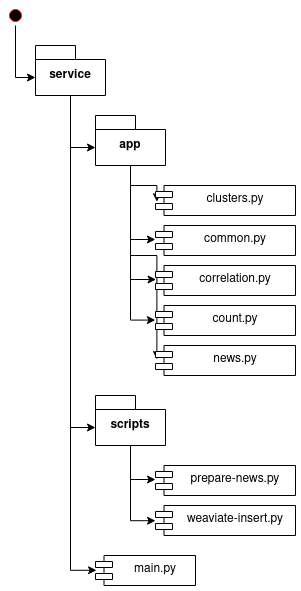
\includegraphics{images/service-struct.png}
    \caption{Общая структура сервиса}
    \label{img:service-struct}
\end{figure}

В директории app находятся основные модули проекта, которые отвечают за выполнение различных задач, таких как расчет корреляции или кластеризацию новостей. В директории scripts находятся вспомогательные скрипты, такие как скрипт добавления данных в базу данных Weaviate. Файл main.py является точкой входа в приложение, реализующей REST API с помощью фреймворка FastAPI. В main.py происходит обработка запросов, а основная логика выполнения запроса осуществляется модулями из директории app.

\subsection{Обработка HTTP-запросов}

На рисунке \ref{img:sequence-diagram} представлена обобщенная диаграмма последовательности выполнения запроса. Обработка HTTP запроса начинаются с экземпляра главного класса FastAPI, который определен в модуле main. В нем содержатся основные настройки сервиса, а также определение конечных точек и маршрутов для запросов. HTTP запрос обрабатывается FastAPI и вызывается соответствующая функция-обработчик, соответствующая маршруту. Из этой функции-обработчика происходит вызов основной логики сервиса, которая выполняет запрос, например, рассчитывает корреляцию. В процессе происходит обращение к векторной базе данных Weaviate для получения новостных данных. Результат запроса возвращается пользователю.

\begin{figure}[h]
    \centering
    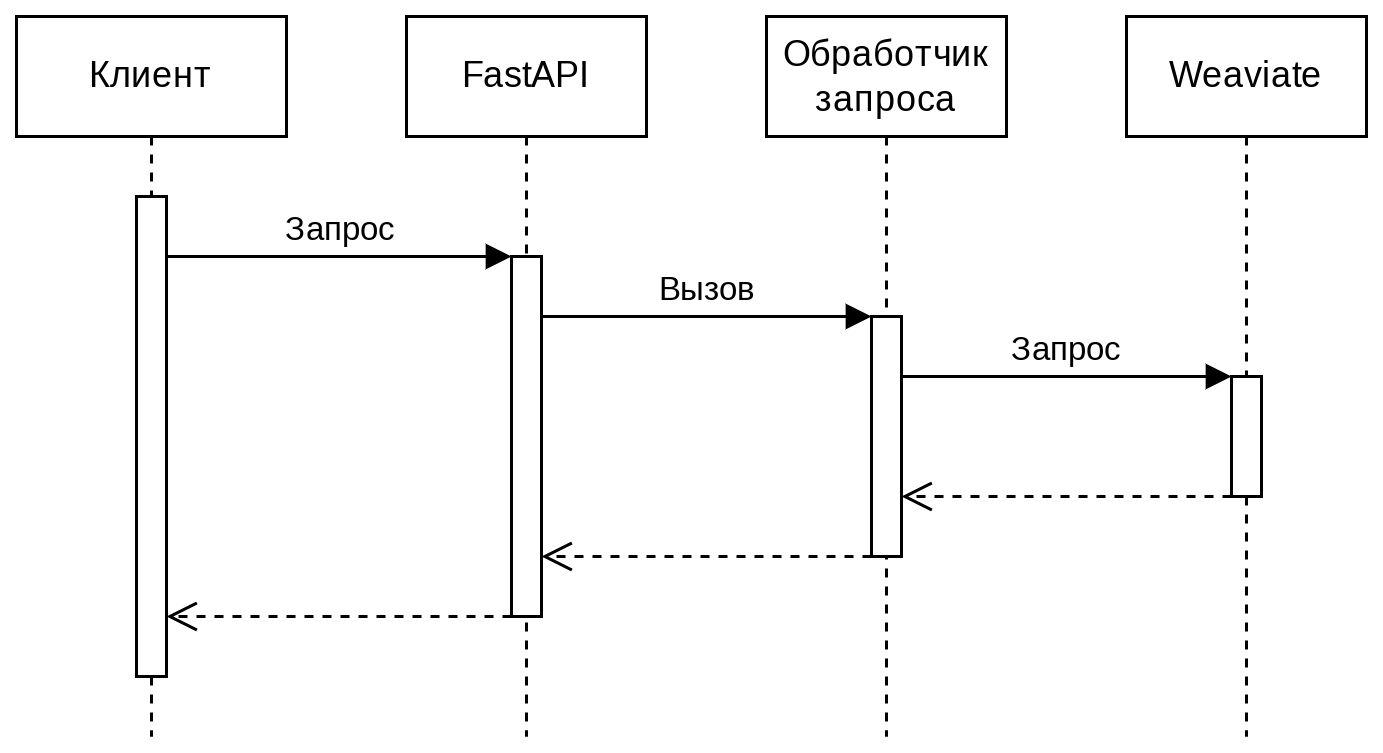
\includegraphics[width=\linewidth]{images/sequence-diagram.png}
    \caption{Диаграмма последовательности обработки запросов}
    \label{img:sequence-diagram}
\end{figure}


Далее приведен пример обработки запроса поиска новостей с помощью семантического поиска.

С помощью декоратора определяется HTTP метод и URL конечной точки API, в данном случае, это GET и адрес <</news>>. Данная функция будет вызвана при получении соответствующего запроса. Параметры функции определяют параметры HTTP запроса. С помощью python type hints указывается тип параметра q: строка. В обработчике запроса происходит вызов функции семантического поиска новостей news\_search.by\_query(), которая возвращает список новостей, полученных из БД, близких к указанному запросу. Затем происходит формирование структуры и возврат ответа. FastAPI автоматически преобразует объект словаря в JSON и отправляет ответ пользователю.

\begin{lstlisting}
@app.get('/news')
def search_news(q: str):
    news = news_search.by_query(q)
    response = {
        'news': news
    }
    return response
\end{lstlisting}

\subsection{Разработка расчёта корреляции}

Основной функциональностью, предоставляемой сервисом, является расчет взаимной корреляции между количеством новостей по определенной теме и предоставленным пользователем временным рядом.

Пользователь указывает в запросе временную метку начала интервала, временную метку конца интервала, длительного шага, интересующую тему новостей и пользовательский временной ряд. Количество элементов пользовательского временного ряда должно совпадать с количеством шагов в указанном временном интервале. Обработка запроса и проверка параметров осуществляется с помощью FastAPI.

Далее осуществляется определение количества новостей по заданной теме за каждый временной шаг. Поиск новостей по указанной теме осуществляется с помощью семантического поиска Weaviate. Необходимо подсчитать количество новостей за указанный временной интервал.

Поиск осуществляется с помощью запроса Aggregate, который позволяет агрегировать результаты поиска различным образом, в данном случае, подсчитать количество найденных новостей. Использование Aggregate позволяет подсчитать количество результатов поиска, не получая сами результаты, которые не требуются.

Для поиска новостей, близких к запросу, используется фильтр nearText, который позволяет отфильтровать результаты на основе векторной близости эмбеддинга новости к эмбеддингу запроса. Данный фильтр принимает параметр concepts, задающий текст запроса, и параметр certainity, определяющий максимальную близость новости к запросу. Certainity определяет требуемую степень сходства характеристик объекта с заданными значениями фильтра. Значения могут быть от 0 (нет совпадения) до 1 (полное совпадение).

Для фильтрации новостей за определенный временной интервал применяется фильтр where, который позволяет применять классическую (невекторную фильтрацию).

Запрос к Weaviate осуществляется с помощью библиотеки weaviate для Python. Ниже приведен код функции, осуществляющий запрос на получение количества новостей, близких к запросу.

Формирование запроса осуществляется с помощью методов класса Client из библиотеки weaviate, которые реализуют паттрен Строитель (Builder). Запрос формируется через цепочку методов, которые добавляют к запросу различные фильтры и параметры.

Рассмотрим формирование и выполнение запроса на получение количества новостей по заданной теме. Функция count\_news имеет следующие аргументы: cleint ~-- объект клиента для работы с Weaviate, start ~-- дата и время начала временного интервала, duration ~-- длительность временного интервала, topic (опционально) ~-- тема новостей. Если параметр topic None, то осуществляется определение общего количества новостей за заданный период, в противном случае, осуществляется определение количества новостей, близких к указанной теме.

Ниже приведен код фильтра, который ограничивает поиск новостей заданным временным интервалом. Фильтр записывает условие $(datetime >= start) and (datetime <= end)$.

\begin{lstlisting}
where_filter = {
    'operator': 'And',
    'operands': [
        {
            'path': ['datetime'],
            'operator': 'GreaterThanEqual',
            'valueInt': int(start.timestamp()),
        },
        {
            'path': ['datetime'],
            'operator': 'LessThan',
            'valueInt': int(end.timestamp()),
        }
    ]
}
\end{lstlisting}

Ниже приведен код составление и выполнение запроса с помощью цепочки методов. В случае, если тема указана, то в запрос добавляется векторный фильтр with\_near\_text, который осуществляет семантический поиск близких к запросу новостей.

\begin{lstlisting}
query = client.query \
    .aggregate('News2') \
    .with_where(where_filter) \

if topic is not None:
    near_text = {
        'concepts': [topic],
        'certainty': CERTAINITY,
    }
    query = query \
        .with_near_text(near_text)

res = query \
    .with_fields("meta {count}") \
    .do()
\end{lstlisting}

Рассмотренная процедура получение количества новостей близких к запросу за заданный промежуток времени повторяется для каждого окна в заданном пользователе временном интервале. Количество новостей за определенное окно, например, за семь дней, является одним элементом временного ряда количества новостей (точкой на графике). После определения количества новостей за окно, окно сдвигается на определенную величину, например, на шесть часов. Повторяя эту процедуру для всего временного интервала, получим набор значений, которые составляют временной ряд количества новостей.

Далее происходит расчёт кросс-корреляции между полученным временным рядом количества новостей и переданным в запросе пользовательским временным рядом. Кросс-корреляция рассчитывается по окнам ~-- весь временной интервал разбивается на несколько непересекающихся окон, для каждого осуществляется расчёт кросс-корреляции. В результате получается временной ряд, который показывает, какая была корреляция между количеством новостей и пользовательским временным рядом в различные моменты времени. Кросс-корреляция рассчитывается по формуле (\ref{eq:cross-corr}).

\begin{equation}
    R(l) = \sum_{i=0}^{N-1}{f(lN+i)g(lN+i)}
    \label{eq:cross-corr}
\end{equation}

\noindent\begin{tabularx}{\linewidth}{lllX}
    где & $R(l)$   &~--& значение корреляционной функции, \\
        & $l$      &~--& номер окна, \\
        & $f$, $g$ &~--& сигналы, \\
        & $i$      &~--& номер отсчёта, \\
        & $N$      &~--& количество отсчётов в окне $l$. \\
\end{tabularx}

Результат расчёта кросс-корреляции отправляется обратно пользователю в ответ на запрос.

\subsection{Разработка метода определения основных новостей}

Для выявления популярных и похожих новостей в работе была применена кластеризация. Идея этого решения заключается в следующем. Существуют новости, описывающие одно событие разными словами, либо новости, описывающие похожие или связанные события, либо новости, относящиеся к одной категории или теме. Т.к. эти новости семантически близки друг к другу, их текстовые эмбеддинги также должны быть близки. Разбивая множество эмбеддингов новостей на кластеры, состоящие из близких друг к другу новостей, мы получаем возможность выявлять группы связанных или близких по теме новостей.

Пользователь указывает в запросе временную метку начала интервала, временную метку конца интервала, для которого необходимо проанализировать новости.

Далее осуществляется получение новостей и их эмбеддингов из базы данных Weaviate за указанный временной интервал. Поиск осуществляется с помощью запроса Get{}, позволяющего получать и фильтровать данные. Для фильтрации новостей за определенный временной интервал применяется фильтр where, который позволяет применять классическую (невекторную фильтрацию). Запрос к Weaviate осуществляется с помощью библиотеки weaviate для Python. Ниже приведен код функции, осуществляющий запрос на получение новостей их эмбеддингов за указанный временной интервал.

\begin{lstlisting}
def get_news_by_timeframe(client, start, end):
    where_filter = {
        'operator': 'And',
        'operands': [
            {
                'path': ['datetime'],
                'operator': 'GreaterThanEqual',
                'valueInt': int(start.timestamp()),
            },
            {
                'path': ['datetime'],
                'operator': 'LessThan',
                'valueInt': int(end.timestamp()),
            }
        ]
    }

    res = client.query \
        .get('News2', ['title']) \
        .with_where(where_filter) \
        .with_additional(['vector']) \
        .with_limit(5000) \
        .do()
    return res['data']['Get']['News2']
\end{lstlisting}

После того, как новости и их эмбеддинги получены, осуществляется кластеризация эмбеддингов. В данной работе применяется алгоритм кластеризации DBSCAN. Это алгоритм density-based кластеризации. Особенностями этого алгоритма являются:
\begin{itemize}
    \item обнаружение кластеров сложной и невыпуклой формы;
    \item работа с кластерами разного размера;
    \item обнаружение выбросов (элементов, не входящих ни в один из кластеров).
\end{itemize}

Широко используемый алгоритм k-means разбивает множество точек с помощью гиперплоскостей, таким образом, кластеры ограничены иметь выпуклую форму. Неизвестно, какую форму имеют кластеры эмбеддингов похожих новостей, поскольку они представлены в 384-мерном пространстве, и могут ли они быть разделены с помощью алгоритма K-Means. Поэтому, был выбран более гибкий и устойчивый алгоритм DBSCAN, который позволяет определять кластеры сложной формы. Помимо этого, DBSCAN не требует указания количества кластеров, а требует указание минимальной требуемой плотности. Недостатком этого алгоритма является соединение нескольких кластеров в один через тонкие <<перемычки>> между ними.

Кластеризация реализована с помощью библиотечных методов из библиотеки scikit-learn. В результате, получается набор кластеров и новостей, входящих в каждый кластер. Список кластеров и содержащихся в них ID новостей возвращаются обратно пользователю в ответ на запрос.
